\documentclass[12pt]{article}
% We can write notes using the percent symbol!
% The first line above is to announce we are beginning a document, an article in this case, and we want the default font size to be 12pt
\usepackage[utf8]{inputenc}
% This is a package to accept utf8 input.  I normally do not use it in my documents, but it was here by default in Overleaf.
\usepackage{amsmath}
\usepackage{amssymb}
\usepackage{amsthm}
% These three packages are from the American Mathematical Society and includes all of the important symbols and operations 
\usepackage{fullpage}
% By default, an article has some vary large margins to fit the smaller page format.  This allows us to use more standard margins.
\usepackage{graphicx}

\setlength{\parskip}{1em}
% This gives us a full line break when we write a new paragraph


\begin{document}
% Once we have all of our packages and setting announced, we need to begin our document.  You will notice that at the end of the writing there is an end document statements.  Many options use this begin and end syntax.

\graphicspath{{figures/}}

\begin{center}
    Tarea 2 \\
    Nahuel Almeira
\end{center}

\begin{center}
    \Large - \normalsize
\end{center}

\section{Ecuaci\'on de onda}

En esta pr\'actica resolvemos la ecuaci\'on de onda en dimensi\'on $D = 1$

\begin{equation}
\dfrac{\partial^2 \phi}{\partial t^2} = v^2 \dfrac{\partial^2 \phi}{\partial x^2}.
\end{equation}

La misma pued reducirse a un sistema de dos ecuaciones desacopladas con derivadas de primer orden. Definimos para ello $W \equiv (w_1, w_2)^T$, donde

\begin{align}
w_1 &= \phi_x \\
w_2 &= \phi_t.
\end{align}

As\'i, la ecuaci\'on se puede expresar como

\begin{equation}
\begin{pmatrix}
\partial_t w_1 \\
\partial_t w_2
\end{pmatrix} = 
\begin{pmatrix}
0 & 1 \\
v^2 & 0
\end{pmatrix} \cdot
\begin{pmatrix}
\partial_x w_1 \\
\partial_x w_2
\end{pmatrix}.
\end{equation}

Es decir,

\begin{equation} \label{eq:wave_1d_system}
\partial_t W = A \cdot \partial_x W,\quad 
A = \begin{pmatrix}
0 & 1 \\
v^2 & 0
\end{pmatrix}.
\end{equation}

Para resolver este sistema, debemos diagonalizar la matriz $A$. Para ello, definimos

\begin{equation}
S = \dfrac{1}{\sqrt{2}}
\begin{pmatrix}
v^{-1} & -v^{-1} \\
1 & 1
\end{pmatrix} \quad \text{y} \quad
S^{-1} = \dfrac{1}{\sqrt{2}} 
\begin{pmatrix}
v & 1 \\
-v & 1
\end{pmatrix}.
\end{equation}

Notemos que la matriz $A$ se puede expresar como una matriz diagonal mediante la transformaci\'on 

\begin{equation}
S^{-1} A S = \Lambda = \begin{pmatrix}
v & 0 \\
0 & -v
\end{pmatrix}
\end{equation}

Multiplicando \ref{eq:wave_1d_system} por $S^{-1}$,

\begin{align*}
S^{-1} \partial_t W &= S^{-1} A \partial_x W \\
\partial_t \left( S^{-1} W \right) &= S^{-1} A S S^{-1} \partial_x W \\
\partial_t \left( S^{-1} W \right) &= \Lambda \partial_x \left( S^{-1} W \right), \\
\end{align*}

donde 

\begin{equation}
\left( S^{-1} W \right) = \dfrac{1}{\sqrt{2}} 
\begin{pmatrix}
v w_1 + w_2 \\
-v w_1 + w_2
\end{pmatrix} =
\dfrac{1}{\sqrt{2}} 
\begin{pmatrix}
v \phi_x + \phi_t \\
-v \phi_x + \phi_t
\end{pmatrix}. 
\end{equation}

Definiendo $U$ y $V$ tal que $(U, V)^T = (S^{-1}W)$, obtenemos el sistema diagonal

\begin{equation}
\begin{pmatrix}
V_t \\
U_t
\end{pmatrix} = 
\begin{pmatrix}
v & 0 \\
0 & -v
\end{pmatrix} \cdot
\begin{pmatrix}
V_x \\
U_x
\end{pmatrix}
\end{equation}

Resolveremos el sistema con la condici\'on inicial $V(t=0) = 0$, lo cual implica que $V(t, x) = 0$. Es decir, resolveremos la ecuaci\'on de advecci\'on

\begin{equation}\label{eq:adv}
U_t = - v U_x.
\end{equation}

Adem\'as, simplificaremos el problema definiendo $v = 1$. Utilizaremos condiciones de contorno peri\'odicas en el dominio $x\in [0,1]$ y dos datos iniciales $U(t=0)$. Los datos iniciales son los siguientes:

\begin{itemize}
\item \textbf{Simple Bump:} 

\begin{equation}
U(x, t=0) = (0.25)^{8}(x - 0.25)^4 (x - 0.75)^4.
\end{equation}

\item \textbf{Square Bump:} 

\begin{equation}
U(x, t=0) = 
\begin{cases}
0 & x < 0.25,\\
(0.05)^8(x-0.25)^4 (x-0.35)^4 & 0.25 \leq x \leq 0.3, \\
1 & 0.3 < x < 0.6, \\
(0.05)^8(x-0.65)^4 (x-0.75)^4 & 0.6 \leq x \leq 0.75, \\
0 & 0.75 < x.
\end{cases}
\end{equation}

\end{itemize}

\section{Soluci\'on exacta}

A continuaci\'on utilizamos la teor\'ia de Fourier para hallar la soluci\'on exacta del problema

\begin{align} \label{eq:system}
U_t &= v U_x,\quad x\in (0, 1), \quad t > 0 \nonumber \\
U(x, t=0) &= f(x)\\
U(0, t) &= U(1, t). \nonumber
\end{align}

El dato inicial $f(x)$ es tambi\'en 1-peri\'odico, es decir, $f(x+1) = f(x)$. Luego, podemos utilizar su expansi\'on en serie de Fourier

\begin{equation}
U(x,t=0) = f(x) = \sum_{-\infty}^{\infty} e^{2\pi i \omega x} \hat{f}(\omega).
\end{equation}

Aplicando separaci\'on de variables, proponemos el ansatz

\begin{equation}
U(x,t) =  \sum_{-\infty}^{\infty} e^{2\pi i \omega x} \hat{U}(\omega, t).
\end{equation}

Derivando respecto a $x$,

\begin{equation}
U_x(x,t) = \sum_{-\infty}^{\infty} 2\pi i \omega x e^{2\pi i \omega x} \hat{U}(\omega, t).
\end{equation}

Por otro lado, derivando respecto a $t$,

\begin{equation}
U_t(x,t) = \sum_{-\infty}^{\infty} e^{2\pi i \omega x} \hat{U}_t(\omega, t).
\end{equation}

Reemplazando en \ref{eq:adv},

\begin{equation}
\sum_{-\infty}^{\infty} e^{2\pi i \omega x} \hat{U}_t(\omega, t) = \sum_{-\infty}^{\infty} 2\pi i \omega x e^{2\pi i \omega x} \hat{U}(\omega, t).
\end{equation}

Teniendo en cuenta la ortogonalidad de las funciones exponenciales, la ecuaci\'on anterior implica que 

\begin{equation}
\hat{U}_t(\omega, t) = 2 \pi i \omega x \hat{U}(\omega, t), \;\forall \omega.
\end{equation}

Teniendo en cuenta el dato inicial, la ecuaci\'on anterior tiene como soluci\'on

\begin{equation}
\hat{U}(\omega, t) = e^{-2\pi i \omega v t} \hat{f}(\omega).
\end{equation}

Por lo tanto, la soluci\'on al problema es 

\begin{equation}
U(x,t) = \sum_{-\infty}^{\infty} e^{2\pi i \omega (x-vt)} \hat{f}(\omega).
\end{equation}

Es decir, la soluci\'on es una onda viajera que conserva la forma inicial, pero que se desplaza con velocidad constante $v$.

\section{Conservaci\'on de la energ\'ia}

\subsection{Caso anal\'itico}

La energ\'ia se define como 

\begin{equation}
E(t) = \int_0^1 U^2(x,t)\; dx.
\end{equation}

Derivando respecto al tiempo,

\begin{equation} \label{eq:E1}
\dot{E}(t) = 2 \int_0^1 U U_t\; dx = -2 \int_0^1 U U_x \; dx,
\end{equation}

donde utilizamos la ecuaci\'on \ref{eq:adv}. Integrando por partes, obtenemos

\begin{equation} \label{eq:E2}
\dot{E}(t) = -2 U(x,t)\big|_{x=0}^{x=1} + 2 \int_0^1 U_x U \;dx.
\end{equation}

Por las condiciones de contorno, $U(1, t) = U(0,t)$. Luego, de \ref{eq:E1} y \ref{eq:E2} tenemos que $\dot{E}(t) = 0$, por lo que la energ\'ia es constante y, por lo tanto, una cantidad conservada.

\subsection{Caso num\'erico}

Definimos el producto interno eucl\'ideo (y su respectiva norma) para funciones de grilla como

\begin{align}
(u,v)_{\ell, m} &\equiv h \sum_{j=l}^m u_j w_j \\
||u||_{\ell, m}^2 &\equiv (u,u)_{\ell, m}.
\end{align}

Utilizando el m\'etodo del trapecio para integrar, la energ\'ia del sistema puede escribirse como

\begin{equation}
E(t) = h\sum_{j=1}^{N-1} U_j^2 + \dfrac{h}{2} (U_0 + U_N).
\end{equation}

Utilizando la periodicidad, tenemos que $U_0 = U_N$, por lo que podemos simplificar la expresi\'on anterior como

\begin{equation}
E(t) \simeq h\sum_{j=0}^{N-1} U_j^2 = (U,U)_{0,N-1}.
\end{equation}

Consideremos, por simplicidad, la derivada espacial discreta de orden 2 

\begin{equation}
D_0 = \dfrac{D_+ + D_-}{2},
\end{equation}

y veamos que la energ\'ia se conserva (lo mismo puede hacerse para derivadas centradas de \'ordenes superiores). Siguiendo la referencia \cite{Kreiss-Ortiz}, tenemos que 

\begin{equation} \label{eq:product_rule}
(u, D_0 v)_{l,m} + (D_0 u, v)_{l,m} = \dfrac{h}{2} \bigg[ u_j v_{j+1} + u_{j+1} v_j \bigg]\bigg|_{l-1}^m.
\end{equation}

Derivando la energ\'ia,

\begin{equation}
\dot{E}(t) \simeq 2 h \sum_{j=0}^{N-1} U_j \partial_t U_j = -2 h \sum_{j=0}^{N-1} U_j D_0 U_j = -2 (D_0 U, U)_{0,N-1}.
\end{equation}

De acuerdo con \ref{eq:product_rule}, tenemos que 

\begin{align}
\dot{E}(t) &\simeq -\dfrac{h}{2}  \bigg[ U_j U_{j+1} + U_{j+1} U_j \bigg]\bigg|_{-1}^{N-1} \\
&\simeq -h   \bigg[ U_j U_{j+1}\bigg]\bigg|_{N-1}^{N-1} = 0.
\end{align}

\section{M\'etodo de las l\'ineas}

El m\'etodo de las l\'ineas consiste en resolver el problema \ref{eq:system} discretizando s\'olo las coordenadas espaciales, pero manteniendo el tiempo continuo, para transformar de ese modo el problema original en un sistema de ecuaciones diferenciales ordinarias, que pueden ser resueltas por m\'etodos est\'andar, como por ejemplo, m\'etodos Runge-Kutta.

Sea $M$ un entero y $h = (2 M +1)^{-1}$ el ancho de grilla, que define los puntos $x_j = hj$, $j=0,\pm 1,\pm 2, \dots$. Aproximamos el problema \ref{eq:system} como

\begin{align}
U_t(x_j, t) &= v D_x^p U(x_j, t) \nonumber \\
U(x_j, 0) &= f(x_j) \\
U(x_0,t) &= U(x_{2M+1},t) \nonumber,
\end{align}

donde $D_x^p$ representa la aproximaci\'on de $\partial/\partial x$ a orden $p$.

Proponemos una soluci\'on de tipo onda simple 

\begin{align*}
U(x_j,t) &= \hat{U}(\omega, t) e^{2\pi i \omega x_j} \\
U(x_j, 0) &= \hat{f}(\omega).
\end{align*}

Reemplazando en la ecuaci\'on, tenemos

\begin{equation}
U_t(x_j, t) =  v\hat{U}(\omega, t) q(\omega) e^{2\pi i \omega x_j},
\end{equation}

donde $q(\omega)$ es el autovalor de $D_x^p$ correspondiente al autovector $e^{2\pi i \omega x_j}$ (tambi\'en llamado \emph{factor de amplificaci\'on}), es decir, 

\begin{equation}
D_x^p e^{2\pi i \omega x_j} = q(\omega) e^{2\pi i \omega x_j}.
\end{equation}

La soluci\'on queda entonces de la forma 

\begin{equation}
U(x_j,t) = \hat{f}(\omega) e^{2\pi i \omega x_j + v q(\omega) t}.
\end{equation}

Comparando con la soluci\'on exacta, vemos que esta soluci\'on aproximada corresponde a una onda plana que se desplaza a una velocidad 

\begin{equation}
\tilde{v}(\omega) = \dfrac{q(\omega)}{2\pi i\omega} v.
\end{equation}

Es decir, la velocidad de la soluci\'on aproximada depende expl\'icitamente de la frecuencia a trav\'es del factor de amplificaci\'on.

La generalizaci\'on de la soluci\'on a cualquier dato peri\'odico $f(x)$ es 

\begin{equation} \label{eq:sol_general}
U(x_j, t) = \sum_{\omega=-M}^M \hat{f}(\omega)  e^{2\pi i \omega x_j + v q(\omega) t},
\end{equation}

donde 

\begin{equation}
f(x) =  \sum_{\omega=-M}^M \hat{f}(\omega)  e^{2\pi i \omega x_j}.
\end{equation}

Luego, vemos que la soluci\'on se ir\'a deformando a medida que los distintos modos avancen cada uno con su correspondiente velocidad.

Siguiendo la referencia \cite{Gustafsson}, podemos expresar los operadores de derivadas espaciales como 

\begin{equation}
D_x^p = D_0 \sum_{\nu=0}^{p/2-1} (-1)^{\nu} \alpha_{\nu} (h^2 D_+ D_-)^{\nu},
\end{equation}

donde 

\begin{align*}
\alpha_0 &= 1 \\
\alpha_{\nu} &= \dfrac{\nu}{2(2\nu+1)} \alpha_{\nu-1}, \quad \nu = 1,2,\dots,p/2-1.
\end{align*}

En particular, los operadores utilizados en el c\'odigo corresponden a los \'ordenes $p=2, 4, 6, 8$. Los correspondientes factores de amplificaci\'on son

\begin{align}
q_2(\omega) &=i\dfrac{\sin (2\pi \omega h)}{h} \\
q_4(\omega) &=i\dfrac{\sin (2\pi \omega h)}{h} \bigg[ 1 + \dfrac{2}{3} \sin^2(\pi \omega h) \bigg] \\
q_6(\omega) &=i\dfrac{\sin (2\pi \omega h)}{h} \bigg[ 1 + \dfrac{2}{3} \sin^2(\pi \omega h) + \dfrac{8}{15}\sin^4(\pi \omega h) \bigg] \\
q_8(\omega) &=i\dfrac{\sin (2\pi \omega h)}{h} \bigg[ 1 + \dfrac{2}{3} \sin^2(\pi \omega h) + \dfrac{8}{15}\sin^4(\pi \omega h) + \dfrac{16}{35} \sin^6(\pi \omega h) \bigg].
\end{align}

Como se puede ver en la figura \ref{fig:ampli}, todos los factores de amplificaci\'on se comportan bien para bajas frecuencias, pero inevitablemente fallan a frecuencias mayores. Cuanto mayor sea el orden de la aproximaci\'on, mayor es el rango de frecuencias para el cual $q \sim 1$. 

\begin{figure}
\center
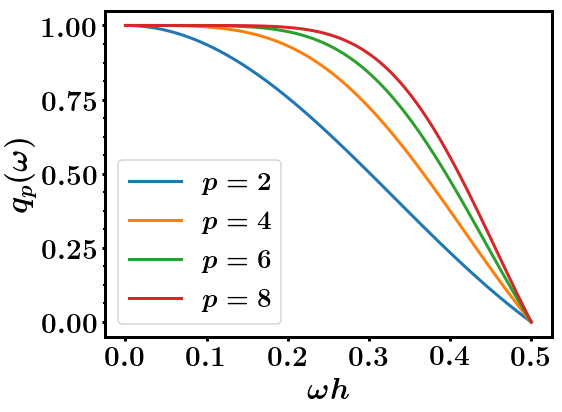
\includegraphics[scale=0.5]{amplification.png}
\caption{Factor de amplificaci\'on en funci\'on de la frecuencia para distintos operadores de derivadas espaciales.} \label{fig:ampli}
\end{figure}

\section{Resultados num\'ericos}

En la figura \ref{fig:simple} mostramos la evoluci\'on de las soluciones aproximadas en funci\'on del tiempo de integraci\'on para el dato inicial \textbf{simple bump}. Como la velocidad es la unidad, las soluciones deber\'ian coincidir con el dato inicial. Podemos ver que la soluci\'on correspondiente a $D_x^2$ comienza a diferenciarse para $T=10$ (ver inset). Las dem\'as aproximaciones se mantienen razonablemente buenas hasta tiempos largos ($T=1000$). 

\begin{figure}
\center
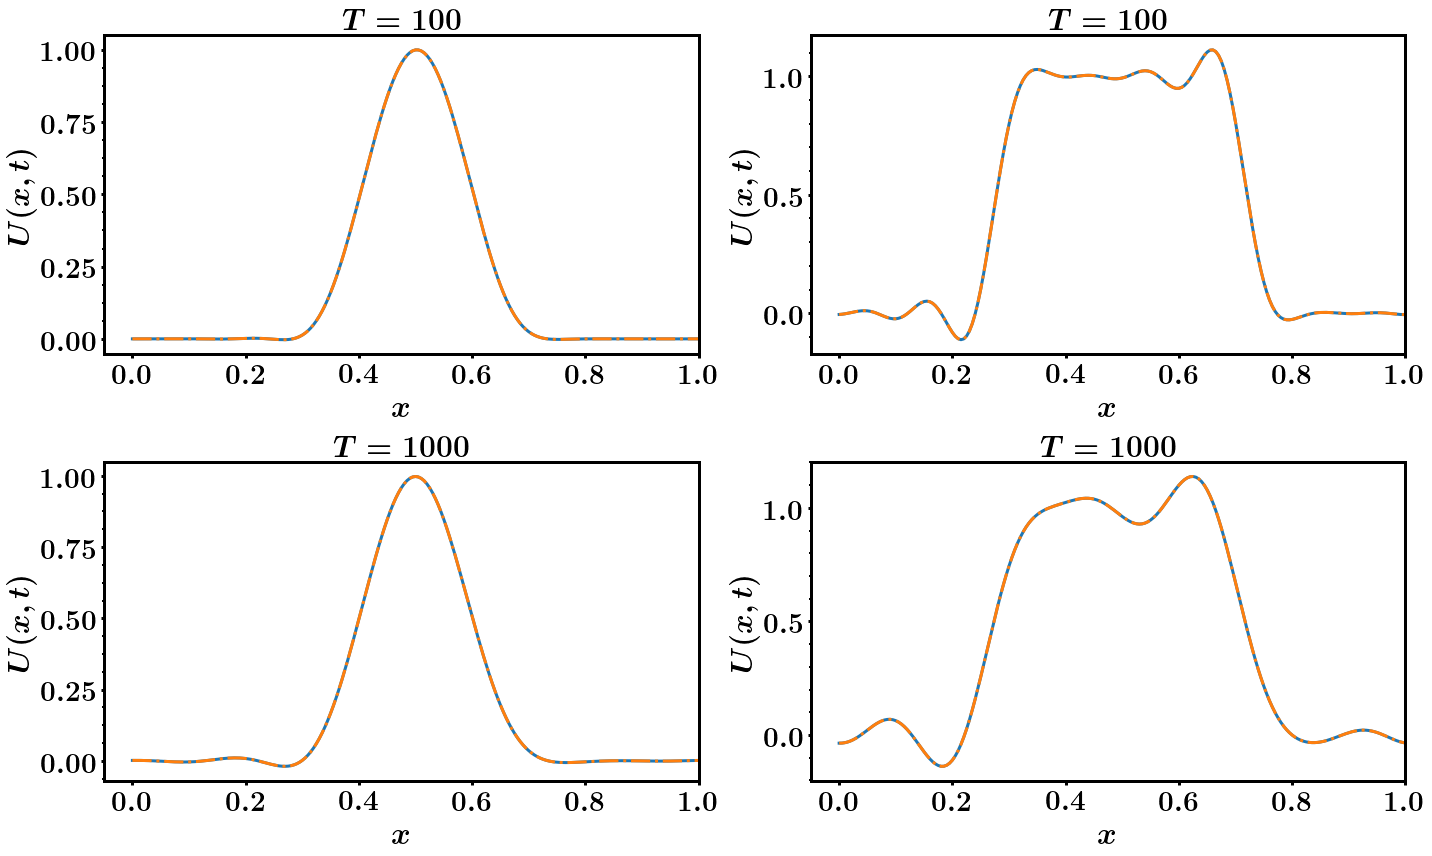
\includegraphics[scale=0.3]{simple.png}
\caption{Comparaci\'on entre las soluciones aproximadas y la soluci\'on anal\'itica para distintos tiempos, para el dato inicial \textbf{simple bump}. $N_x=501$, $\mathrm{CDF} = 0.501$.} \label{fig:simple}
\end{figure}

Para el dato inicial \textbf{square bump}, en cambio, la soluci\'on comienza a deformarse antes (figura \ref{fig:square}). Ya para $T=100$ es posible ver diferencias significativas en la aproximaci\'on $D_x^4$. Para $T=1000$, se ven diferencias en todas las aproximaciones.

\begin{figure}
\center
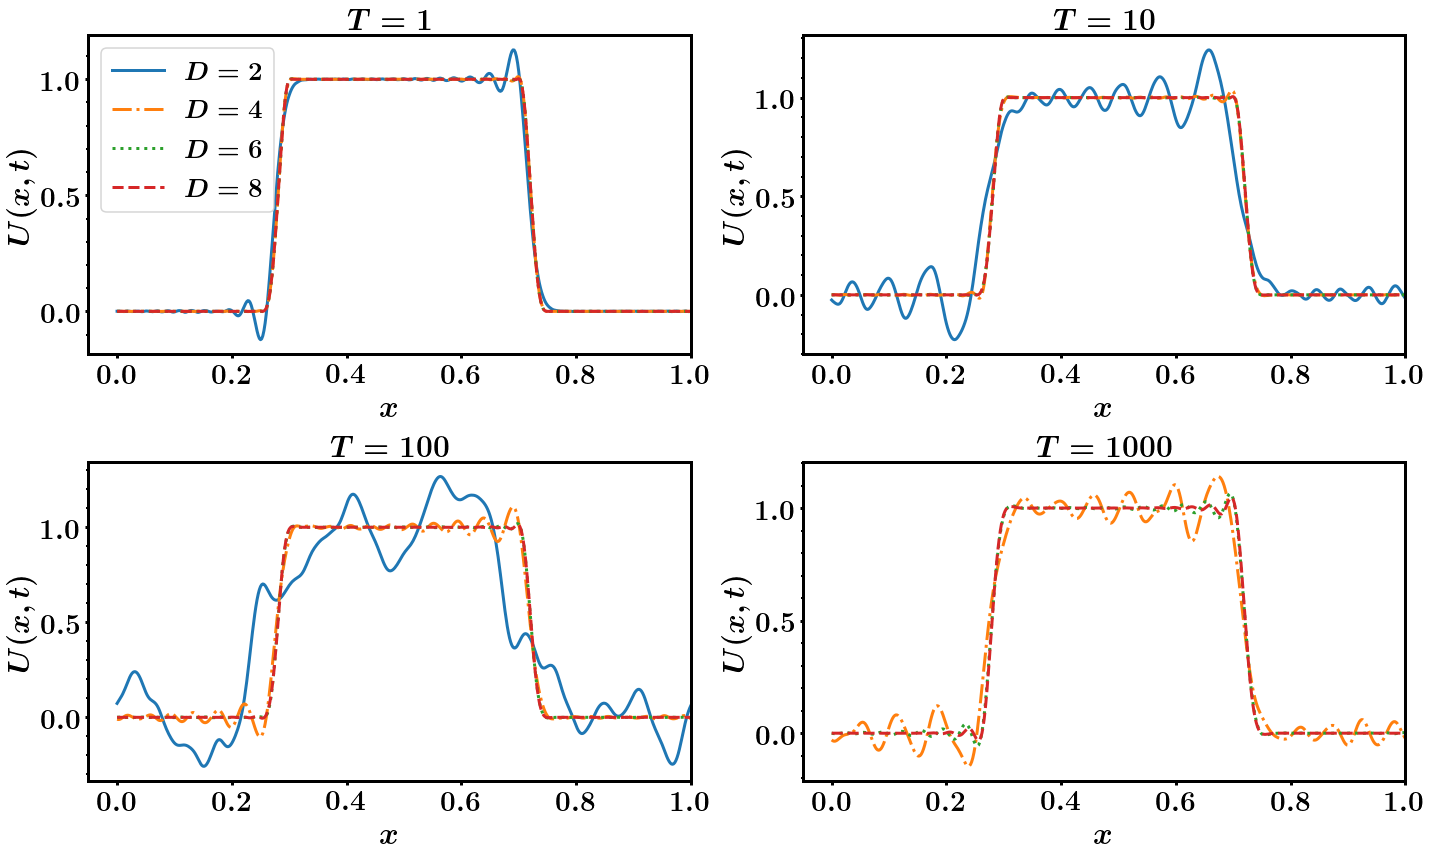
\includegraphics[scale=0.3]{square.png}
\caption{Comparaci\'on entre las soluciones aproximadas y la soluci\'on anal\'itica para distintos tiempos, para el dato inicial \textbf{square bump}. $N_x=501$, $\mathrm{CDF} = 0.501$.} \label{fig:square}
\end{figure}

\subsection{Convergencia y orden de aproximaci\'on}

Analizamos la convergencia del m\'etodo de manera similar a lo realizado en la Tarea 1. Definimos la cantidad $Q(t)$ como

\begin{equation}
Q(t) = \dfrac{||U_{h}(x_j, t) - U_{h/2}(x_j, t)||_{L_q}}{||U_{h/2}(x_j, t) - U_{h/4}(x_j, t)||_{L_q}},
\end{equation}

donde $L_q$ representa una norma espec\'ifica. En este caso, comparamos las normas $L_2$ y $L_{\infty}$. De acuerdo con \cite{Kreiss-Ortiz}, se deber\'ia cumplir que $Q\approx 2^p$. En la figura \ref{fig:convergencia} mostramos el an\'alisis para el operador de segundo orden. Podemos ver que la norma $L_2$ muestra que el m\'etodo funciona correctamente, con el orden de aproximaci\'on correcto. La norma $L_{\infty}$ no coincide con el valor correcto, lo cual no quiere decir que el m\'etodo falle.

\begin{figure}
\center
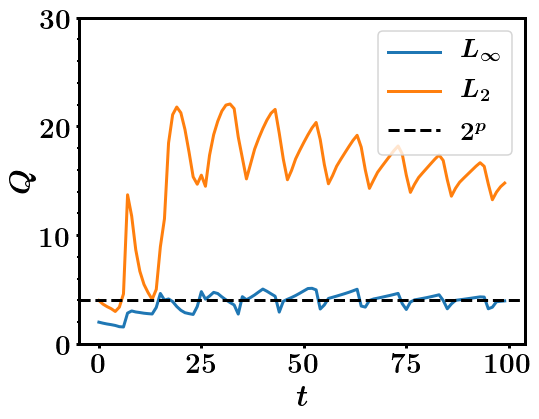
\includegraphics[scale=0.5]{convergencia_tiempo.png}
\caption{An\'alisis del orden de aproximaci\'on del m\'etodo para el dato inicial \textbf{simple bump}. $p=2$, $h =1/400$.} \label{fig:convergencia}
\end{figure}

\subsection{Disipaci\'on}

Para disminuir el error de disipaci\'on en altas frecuencias, una opci\'on es agregar un t\'ermino disipativo de orden superior. En este caso, la ecuaci\'on \ref{eq:system} se transforma en 

\begin{equation}
U_t = v D_x^p U + \sigma D_{xx}^{p+2} U, \quad \sigma > 0.
\end{equation}

El t\'ermino disipativo se encarga de corregir los modos de alta frecuencia a tiempos largos, disminuyendo la deformaci\'on de la onda inicial. 

En la figura \ref{fig:diss}, se puede ver la comparaci\'on entre las soluciones aproximadas utilizando o no la disipaci\'on. Se observa que, con disipaci\'on, la soluci\'on se mantiene m\'as suave. La mejora es casi nula para \textbf{simple bump}, pero bastante notoria para \textbf{square bump}, debido a que tiene una mayor contribuci\'on de altas frecuencias.

\begin{figure}
\center
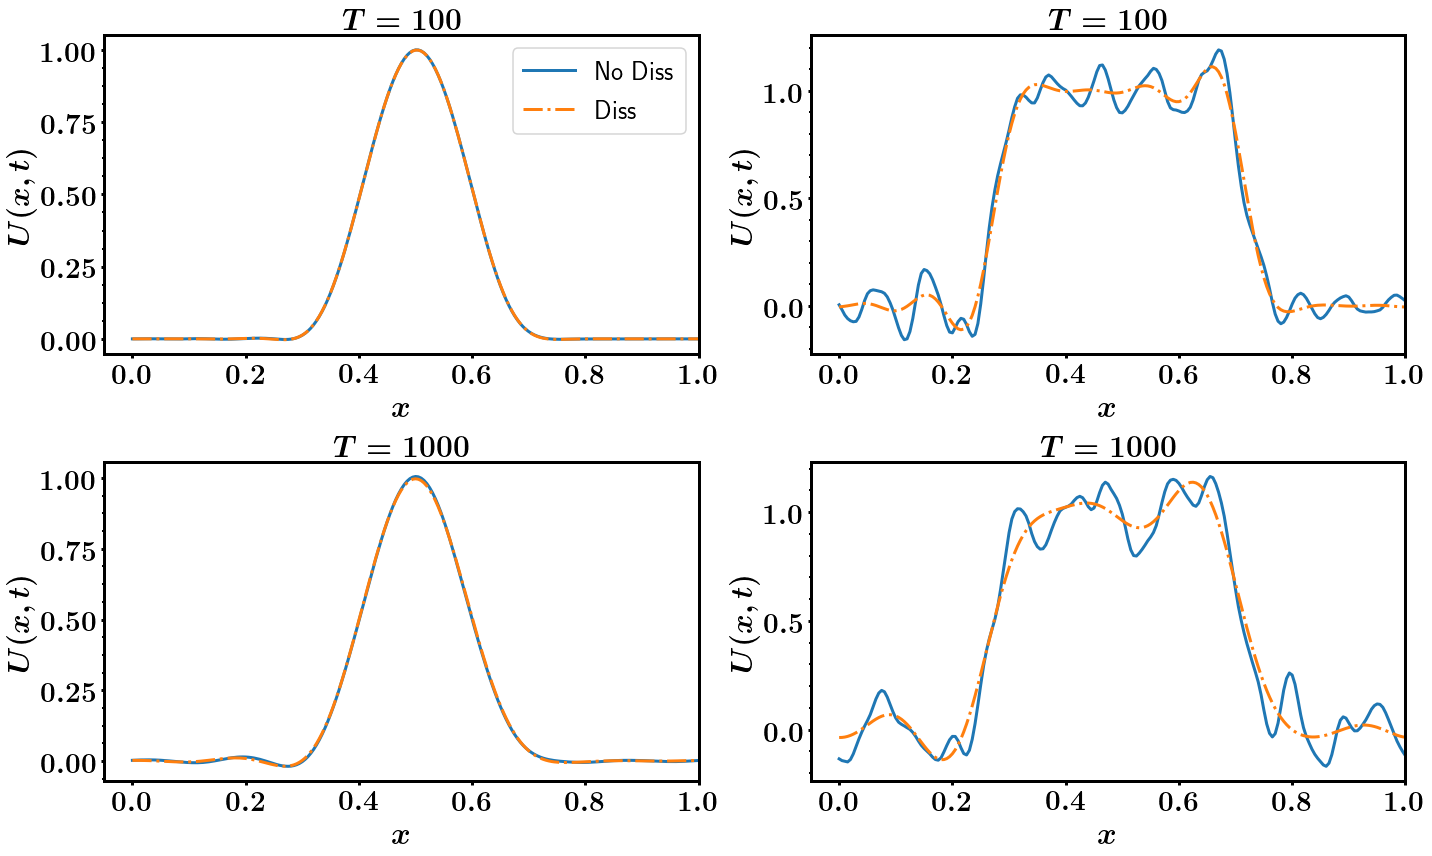
\includegraphics[scale=0.3]{diss.png}
\caption{Comparaci\'on entre las soluciones aproximadas con y sin disipaci\'on, con $p=4$, $N_x=201$ y $\mathrm{CDF} = 0.201$.} \label{fig:diss}
\end{figure}

\subsection{Envolvente de alta frecuencia}

Tomamos el dato \textbf{simple bump} como envolvente de una onda senoidal de alta frecuencia. Concretamente, definimos 

\begin{equation}
U(x, t=0) = (0.25)^{8}(x - 0.25)^4 (x - 0.75)^4 \sin(2\pi \omega_{0}),
\end{equation}

con $\omega_0 = 50$.

Partiendo de la soluci\'on general \ref{eq:sol_general} con $v=1$, y definiendo $k=2\pi \omega$ y $\Omega(k) = q(k/2\pi)/i$, podemos expresar

\begin{equation} \label{eq:paquete}
U(x_j, t) = \sum_{\omega=-M}^M \hat{f}(\omega)  e^{i(k x_j + \Omega) t},
\end{equation}

la cual representa un paquete de ondas. Si las frecuencias est\'an entradas en torno a $k_0$, la velocidad de grupo se define como 

\begin{equation}
v_g = \dfrac{\partial \Omega}{\partial k}\bigg|_{k=k_0}.
\end{equation}

Utilizando las expresiones para los distintos autovalores $q_p$, podemos determinar la velocidad de grupo para cada orden de aproximaci\'on. Por ejemplo, para $p=2$ y $h = 1/400$, tenemos

\begin{equation}
v_g^{(2)} = \dfrac{d}{d (2\pi\omega)}\bigg[ \dfrac{\sin(2\pi\omega h)}{h}\bigg]\bigg|_{\omega = \omega_{0}} = \dfrac{\cos(2\pi\omega_0 h)}{h} = 0.707.
\end{equation}

Del mismo modo, obtenemos

\begin{align}
v_g^{(4)} &= 0.943,\\
v_g^{(6)} &= 0.991,\\
v_g^{(8)} &= 0.998.
\end{align}

Vemos que, cuanto mejor es el orden de aproximaci\'on en la derivada espacial, m\'as se aproxima la velocidad de grupo a la velocidad correspondiente a la soluci\'on anal\'itica (en este caso, la unidad).

En la figura \ref{fig:envolvente} se puede ver c\'omo se produce el retraso para cada uno de los operadores de derivadas espaciales empleados.


\begin{figure}
\center
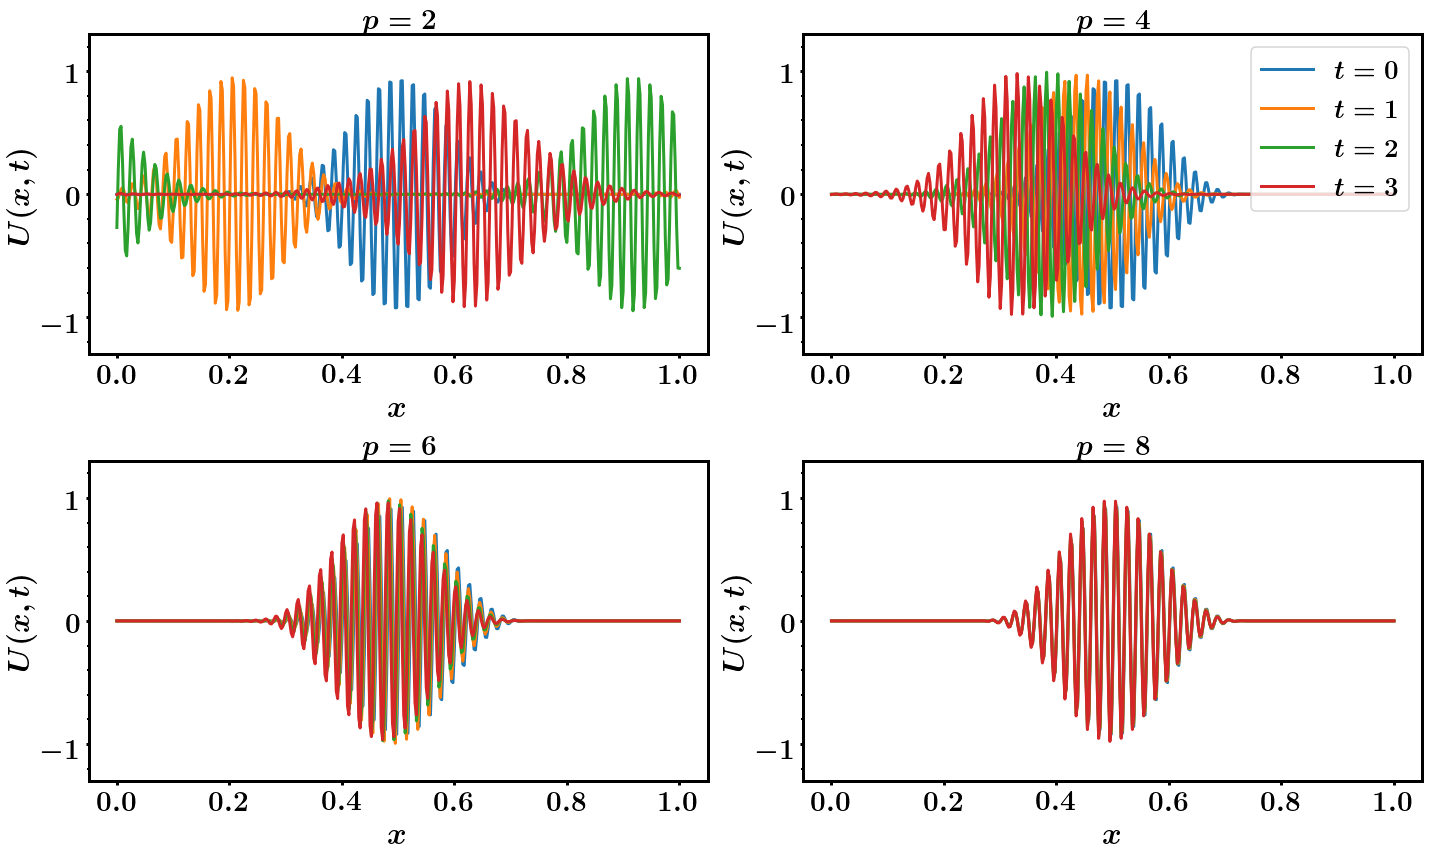
\includegraphics[scale=0.3]{envolvente.png}
\caption{Dato inicial \textbf{simple bump} con envolvente de alta frecuencia ($\omega_0 = 50$).  $N_x=401$ y $\mathrm{CDF} = 0.401$.} \label{fig:envolvente}
\end{figure}


%%%%%%%%%%%%%%%%%%%%%%%%%%%%%%%%%%%%%%%%%%%%%%%%%

\begin{thebibliography}{1}

\bibitem{Kreiss-Ortiz} {\em Introduction to Numerical Methods for Time Dependent Differential Equations}, H. Kreiss and O. Ortiz, (2014).

\bibitem{Gustafsson} {\em High Order Difference Methods for Time Dependent PDE}, B. Gustafsson, (2008).

\end{thebibliography}


\end{document}
